\documentclass[12pt]{article}
\usepackage{url}
\usepackage{amsmath,amsthm,enumitem}
\usepackage{geometry}
\geometry{left=1.5cm, right= 1.5cm, top=2.5cm, bottom=2.5cm}
\usepackage{graphicx}
\usepackage{float}
\usepackage{hyperref}
\usepackage{indentfirst}
\title{CS6630 Project Proposal\\
       Visualization for Flights On-time Performance of the United States}
\author{Run Li, Yulong Liang, Zhi Wang}

\begin{document}

\maketitle

\section{Basic Information}
    $\diamond$ The project title is "Visualization for Flight On-time Performance of the United States".

    $\diamond$ Group members:

    $\quad\cdot$ Run Li, u0879939, $u0879939@utah.edu$

    $\quad\cdot$ Yulong Liang, u1143816, $u1143816@utah.edu$

    $\quad\cdot$ Zhi Wang u0761669, $u0761669@utah.edu$

    $\diamond$ Project repository link: \url{https://github.com/zhiwang93/CS6630Project}

\section{Background and Motivation}

Air travel in the United States has seen a steady rising after the period of post-9/11. By the end of 2016, there were over 5,116 public airports and a total number of 6,676 commercial aircraft in the U.S., which serve more than 2,500,000 passengers everyday.\cite{byTheNumbers}

In 2016, U.S. airlines carried an all-time high number of passengers --- 823.0 million systemwide with 719.0 million domestic and 214 million international, which is 3.1 percent more than the previous record high 798.2 million reached in 2015.\cite{2016data} Moreover, U.S. carrier enplanements are predicted to grow 2.5 percent per year before 2037 according to the Federal Aviation Administration (FAA) Aerospace Forecast.\cite{FAA_A_F}

Despite the rapid growth of aviation industry, the flight on-time performance in U.S. is still unsatisfying: while the percentage of delayed flights fluctuated between 16.7 and 24.1 in the recent 10 years, the average length of delays has increased since 2010 and reached 58.9 minutes in 2015.\cite{PTFF2016}

Although the Department of Transportation (DOT) requires all U.S. airlines to report on operations to and from only the 29 major airports, all the reporting airlines provide their entire domestic data.\cite{airconsumer} These data are published on the website of DOT's Bureau of Transportation Statistics (BTS) for public access.

BTS also summaries and provides monthly reports on the on-time performance of domestic flights. These statistical reports are inclusive and precise but may be too professional and obscure for the public to retrieve information. Moreover, these reports are separated from each other which prevent the readers to have an integrated insight into the data.

In this project, we will explore an instance of visualization of the on-time performance data of all the domestic flights in the United States since 2002. We expect to give people an intuitional view and interactive experience of the data, which can make it easier for the public to discover not only the on-time performance in terms of different regions, airports, carriers, months and time slots but also the relationship between distribution of flights and their spatial and temporal conditions. With this tool, passengers can make better decisions on the selection of airports, flight carriers, departure time and whether to buy a delay insurance or not; airlines can gain a comprehensive and comparative perspective on their operation and aviation authorities can explore the overall performance and make policies to promote the development of the entire aviation industry.

\section{Project Objectives}
    \noindent In this project, we expected to show:\\
    $\diamond$ The connection of each airport to other airports.\\
    $\diamond$ The distribution of flights of each airport in each time period.\\
    $\diamond$ A comparison between planned departing time and actual departing time.\\
    $\diamond$ A comparison between planned arriving time and actual arriving time.\\
    $\diamond$ The rate of diversion and cancellation.\\
    $\diamond$ The temporal and spatial distribution of delayed flights.\\
    $\diamond$ The percentage of causes of delay.\\
    $\diamond$ A view of the time evolution of the flights.

    With these visualizations, we will show how complicated the aviation system is and to reveal some relationship between the distribution of flights and their spatial and temporal conditions. We will see which area has the highest density of flights, which airport is the busiest, at what time we may expect a delayed flight, etc.

\section{Data}
    \noindent We collect our data for the project from several different sources:\\
    $\diamond$ Geography data:\\
    \indent Census Bureau: \url{www.census.gov}\\
    $\diamond$ Airport data:\\
    \indent Federal Aviation Administration (FAA): \url{www.faa.gov}\\
    \indent OpenFlights: \url{openflights.org}\\
    \indent OurAirports: \url{ourairports.com}\\
    $\diamond$ Flight operation data:\\
    \indent Buerau of Transportation Statistics: \url{www.bts.gov}.
    $\diamond$ Real-time flight dynamic data:\\
    \indent FlightAware: \url{www.flightaware.com}.

\section{Data Processing}
    \subsection{Geography data}
    Geography data is designed for the use of d3, so we directly use it without modification.
    
    \subsection{Airport data}
    \begin{enumerate}
    \item Filter out commercial airports which is included in the airlines' on-time performance data report. Group other airports for future use.
    \item Filter out the useless data and extract useful information along with the latitude and longitude for each airport in Step 1.
    \item Join data like annual enplanements, delay rate, mishandled baggage rate, denied boarding rate and number of consumer complaints with Step 2.
    \end{enumerate}
    
    \subsection{Flight operation data}
    \begin{enumerate}
    \item Calculate the elementary data needed such as annual/monthly/daily/hourly flight dencity, expectation of departure/arriving delay time, standard diviation of departure/arriving delay time, proportion of causes of delay, etc. for a specific segment (a departure and destination pair) of a specific airline.
    \item Calculate aggregation data for each airport using the data in Step 1.
    \item Calculate aggregation data for each segment using the data in Step 1.
    \item Calculate aggregation data for each airline using the data in Step 1.
    \item Calculate aggregation data for any combination of airport, segment or airline using the data in Step 1.
    \item Join aggregation operation data with airport data.
    \end{enumerate}

\section{Visualization Design}

The pivot of the visualization will be a map of the United States showing all the commercial airports around the country. These airports are represented by circles of different sizes depending on the level of annual enplanements and different colors depending on the on-time performances of a particular year. In the year chart, users may select the specific year which they want to be visualized. The default year will be the most recent year, in this case, the year of 2016.

On the map, each circle which indicates an airport is interactive. Whenever the user hover onto an airport, a tooltip containing the detail as well as all the flight segments to and from the specific airport will appear. The tooltip information includes the state, city, runway information, airport facilities, annual enplanements, on-time performance, etc. The flight segments information shows all the airports this airport connecting with non-stop flights. The density and on-time performance of a particular segment are represented by the width and color of the path between the two airports.When the user moves the mouse cursor out, the information will disappear unless her/she click on the airport to pin it. A second click will unpin the information. It is also supported to click on several different airports to show the comprehensive information.

Under the map are several elaborate statistical charts which show the annual change, monthly change and change during a day of the on-time performance for particular airport. The cause of delays is also provided under five major categories: air carrier delay, extreme weather delay, national aviation system delay, security delay and late arriving aircraft delay. These charts can also be drawn as the comparison among different years, airports or airlines.

\section{Must-Have Features}
    \subsection{Connections between airports}
    We will visualize the connections between airports with an image similar to the following:
    \begin{figure}[H]
      \centering
      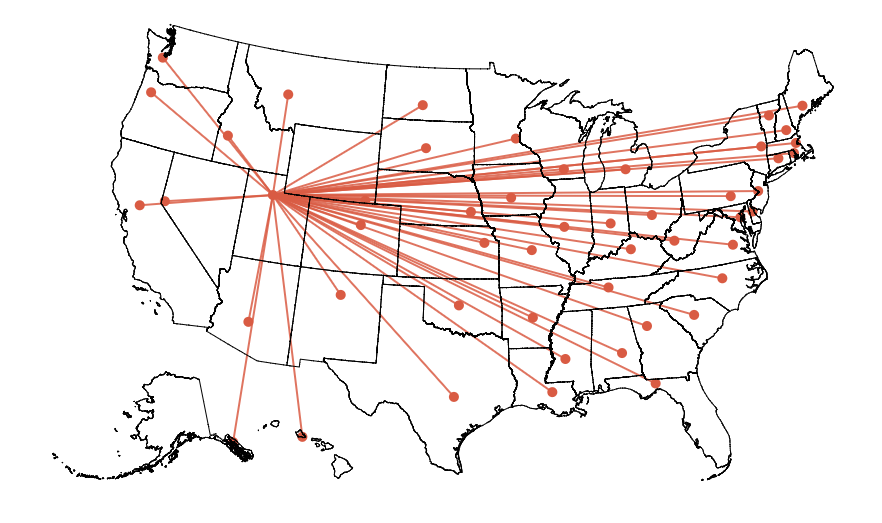
\includegraphics[width=12cm]{G:/CS6630/CS6630Project/proposal/source/airportConnection.PNG}
    \end{figure}
    \noindent The final appearance should be:\\
    $\diamond$ The initial image will show all the airports and highlight some important ones.\\
    $\diamond$ The airports are scaled according to the level of annual enplanements (size of circle) and rate of delay (color of circle).\\
    $\diamond$ When any airport is hovered/selected, it will highlight all the airports which it has flights from or to by a straight line.\\
    $\diamond$ .The line are scaled according to the density of segments (line width) and rate of delay (line color)\\
    $\diamond$ The image will show the name, number of passengers, average delay of the selected airport and other useful related information.\\
    $\diamond$ A year chart will be placed above the chart in order to let readers select the specific year to display. (Default would be the current year.)

    \subsection{statistical charts}
    \noindent $\diamond$ A bar chart to show annual change of the on-time performance of the current airport.\\
    $\diamond$ A bar chart to show monthly change of the on-time performance of the current airport.\\
    $\diamond$ A bar chart to show daily change of the on-time performance of the current airport.\\
    $\diamond$ A pie chart to show the distribution of the causes of flight delay.\\
    $\diamond$ Line charts to show the comparation between the selected airports in terms of years/months/days of a week/time of a day.\\
    $\diamond$ Line charts to show the comparation between the selected airlines and other airlines in terms of years/months/days of a week/time of a day.\\

\section{Optional Features}
    \subsection{Narrative Visualization}
    Come up with a way to visualize the data in a story-telling style, to ease the readers' exploration of the implicit information. 
    \subsection{Dynamic Effects}
    We will add some dynamic effects if possible. For each airline, we will draw the airplane with a small object. It will move back and forth along the airline according to the actual flight time. Then in the image we will be able to overview the running of the whole U.S. aviation system.
    This data is available on website FlightAware.com. It's possible if we can crawl those data down.
    \subsection{Mishandled-Baggage Rate, Denied Boarding Rate \& Consumer Complains}
    To make it more considerable for the aviation consumers to improve understanding over the services provided by different airports and airlines. We will additionally summarize and analyze the Mishandled-Baggage Rate, Denied Boarding Rate and Number of Consumer Complains for each airport and airline respectively.
    \subsection{Tips for the Airport}
    When any of the airports on the map are hovered, it would show some kinds of tips for the overview of an airport. Information displayed includes name, location, enplanement, number of airports connected, rate of delay, etc.
    \subsection{Airport Points Map}
    We will implement a map that is simply composed of circles which indicate more than 18,000 airports in US instead of using a typical US map. Since we have a lot of airport data we may be able to construct the map with the data point (each data will have the location and we use scale to modify the location data for making our own map).
    \subsection{Map Zooming with brush}
    Zoom in/out the map with brush to switch between overall and detailed map.
\section{Project Schedule}
\begin{table}[H]
\center
  \begin{tabular}{c|l}
  \hline
  Week & Assignment\\
  \hline
  1 & Cleanup and extract data\\
  2 & Build the frame and try to implement some basic features \\
  3 & Implement Must-have features \\
  4 & Implement Must-have features \\
  5 & Try to implement optional feature and review\\
  \hline
\end{tabular}
\end{table}



%\cite{2017delay}
%\cite{causes}
%\cite{Corrected}
%\cite{PTTF2015}
%\cite{AnnualReport2016}


\newpage
\renewcommand\refname{Reference}
\bibliographystyle{plain}
\bibliography{Reference}

\end{document}
